\chapter{Evaluierung}\label{kap:eval}

\section{Evaluierungs Metriken}\label{sec:metricen}

\subsection*{Mean Average Precision (mAP)}
Als Maß für die Genauigkeit wird für die Objekterkennung häufig 
die \textit{Mean Average Precision (mAP)} verwendet, welche sowohl
die Lokalisierung- als auch die Klassifizierungsgenauigkeit 
mit einbezieht. Dafür wird zunächst die \textit{Intersection over 
Union} berechnet, welche wie in Abbildung \ref{fig:iou} dargestellt das Verhältnis
des Überlappungsgrad der gelabelten (Ground Truth) und der
geschätzete Boundig Box zu dem Gesammtbereich beider Boxen darstellt.
\\
Beträgt dieser mehr als ein Bestimmter Threshhold, häufig 50\%
gilt die Schätzung als \textit{True Positive}, andernfalls als 
\textit{False Positive}. Werden die Falsschätzungen, also Negative 
noch hinzugenommen, für fälschlicherweise daneben FN und für richtiger 
weise daneben TN, lässt sich daraus eine \textit{Confusion Matrix}
bilden.

% für confusion matrix
\newcommand\MyBox[2]{
  \fbox{\lower0.75cm
    \vbox to 1.7cm{\vfil
      \hbox to 1.7cm{\hfil\parbox{1.4cm}{#1\\#2}\hfil}
      \vfil}%
  }%
}
\noindent
\renewcommand\arraystretch{1.5}
\setlength\tabcolsep{0pt}

\begin{minipage}{\textwidth}
    \begin{minipage}[b]{0.49\textwidth}
      \centering
      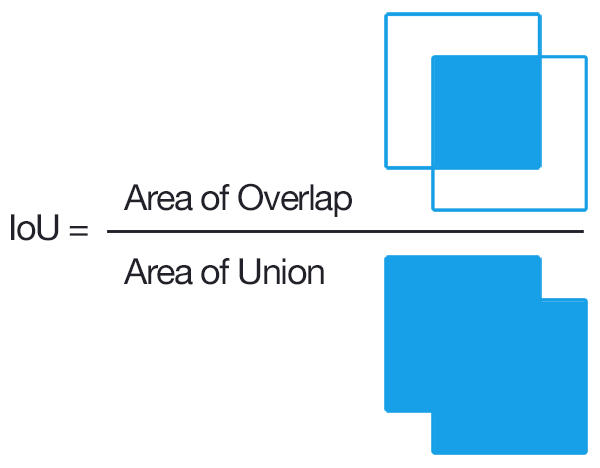
\includegraphics[width=0.8\textwidth]{Bilder/IoU.png}
      \captionof{figure}{Intersection over Union}
    \end{minipage}
    \hfill
    \begin{minipage}[b]{0.49\textwidth}
      \centering
      \begin{tabular}{c >{\bfseries}r @{\hspace{0.7em}}c @{\hspace{0.4em}}c @{\hspace{0.7em}}l}
        \multirow{10}{*}{\rotatebox{90}{\parbox{2.5cm}{\bfseries\centering tatsächlicher Wert}}} & 
          & \multicolumn{2}{c}{\bfseries geschätzter Wert} & \\
        & & \bfseries p & \bfseries n & \bfseries\\
        & p$'$ & \MyBox{True}{Positive} & \MyBox{False}{Negative}\\[2.4em]
        & n$'$ & \MyBox{False}{Positive} & \MyBox{True}{Negative} \\
      \end{tabular}
        \captionof{figure}{Confusion Matrix}
    \end{minipage}
\end{minipage}


\vspace{0.5cm}
    

Mit diesen Werten lassen sich dann der \textit{Recall}, welcher angibt wie 
viele Objekte das Modell gefunden hat und die \textit{Precision}
die angibt mit welcher Genauigkeit die Objekte gefunden wurden
berechnen.
\\
Der \textit{Recall} ist definiert durch TP/TP + FN
wobei TP + FN allen Objekten im Bild entspricht, somit also das 
Verhälltnis der Gefunden zu allen Objekten im Bild.
\\
Die \textit{Precision} kann durch TP/TP + FP, also die richtig 
geschätzen durch alle gemachten schätzunge und gibt somit die 
genauigkeit mit der das Model die Objekte findet an.
\\
Daraus kann nun die durchschnittliche Precision für alle Recall 
Werte bestimmt werden, welche als \textit{Average Precision}
bezeichnet wird und die Genauigkeit des Models bezogen auf 
eine bestimmte Klasse angibt. Für alle Klassen gemittel 
erhält man die mittlere durchschnittliche Precision (mAP)


\subsection*{Fehlerfunktion (Loss)}
Die Fehlerfunktion setzet sich aus einem Lokalisierungs und einem 
Klassifizierungsfehler zusammen. 
Die Lokalisierung erfolgt über eine Lineare Regression zur 
Annäherung der Bounding Boxes and die richtigen Koordinaten.\\

Bei Faster R-CNN werden diese beiden Loss Werte dann sowohl für 
RPN(1st stage) als auch für classifier(2nd stage) also 
insgesammt 4 loss werte verwendet.

\section{Ergebnisse}\label{sec:results}
im Folgenden die Ergebnisse aus \ref{kap:object_det} anhand der 
Metriken sowie Inferenz zeit verglichen und ausgewertet.


\subsection{Modell Vergleich}\label{sec:model_vergl}

Vergleich SSD Mobilenet/Inception mit Faster R-CNN: Inception/(Resnet)
wenn nativ supported von openvino, sonst nicht. bezogen auf sowohl 
mAP, Loss, und Infer FPS


\subsection{Regularisierung}\label{subsec:regularisierung}


Zum Vergleich der Loss ohne Augmentierung nimmt stark zu. Mit Overfitting 
wird am aktuellen Wert angehalten, der mAP kann jedoch seinen Endwert nicht 
erreichen. mit Aumentierung bleibt der Loss klein, nimmt jedoch nach
vielen Schritten auch wieder zu.


\begin{minipage}[t]{0.5\textwidth}
    \centering
    \label{fig:speed_acc}
    \def\svgwidth{0.9\textwidth}
    \input{Bilder/overfitting_kein_early_aug_mAP.pdf_tex}
    %\captionof{figure}{mAP}
\end{minipage}
\begin{minipage}[t]{0.5\textwidth}
    \centering
    \label{fig:speed_acc}
    \def\svgwidth{0.9\textwidth}
    \input{Bilder/overfitting_kein_early_aug_loss.pdf_tex}
    %\captionof{figure}{loss}
\end{minipage}


durch l2 regularisierung an der ersten stufe (rpn), konnte 
der Objecness loss (orange kurve) verbessert werden (blaue kurve)



\begin{minipage}[t]{0.5\textwidth}
    \centering
    \label{fig:speed_acc}
    \def\svgwidth{0.9\textwidth}
    \input{Bilder/overfitting_aug_and_l2_mAP.pdf_tex}
    %\captionof{figure}{mAP}
\end{minipage}
\begin{minipage}[t]{0.5\textwidth}
    \centering
    \label{fig:speed_acc}
    \def\svgwidth{0.9\textwidth}
    \input{Bilder/overfitting_aug_and_l2_objectness_loss.pdf_tex}
    %\captionof{figure}{loss}
\end{minipage}


eine übersicht über alle verwendeten regularisierungsmechanismen ist in 
Tabelle \ref{tab:overfitting} dargestellt.

\begin{table}[htb]
    \begin{tabular}{lcc}
                                                             & mAP & Loss \\ \hline
    \multicolumn{1}{l|}{keine}                               & 0,67  & 0,82   \\ \hline
    \multicolumn{1}{l|}{Early Stopping}                      & 0,67  & 0,69  \\ \hline
    \multicolumn{1}{l|}{Augmentierung}                       & 0,7 & 0,74  \\
    \multicolumn{1}{l|}{\quad +Dropout}       & 0,7 & 0,73 \\
    \multicolumn{1}{l|}{\quad +L2 Reg (0.01)} & 0,7  & 0,69  \\
    \multicolumn{1}{l|}{\quad +L2 Reg (0.02)} & 0,69 & 0,7 \\\hline
    \end{tabular}
    \label{tab:overfitting}
    \caption{Vergleich verschiedener Regul.}
\end{table}




% \subsection{Dataset Distributions}\label{subsec:distributions}
% Da sowohl trainings als auch eval daten aus dem web bezogen wurden,
% also der gleichen distribution sind, diese aber nicht unbedingt 
% den realen bedingungen entsprechen, wurde ein weiteres Evaluierungs 
% Set mit Eigenen Aufnahmen erstellt, welche, da in der Umgebung 
% (Wiltierpark in Reutlingen) aufgenommen, der tatsächlichen daten 
% wahrschverteilung eher entspricht.
% \\
% ergebnisse tabellarisch vergleichen: handy vs orig für die in 
% \ref{subsec:regularization} beschriebenen Regularisierungs techniken\\
% wenn für Augmentierung besser, heist das Augmentierung ist besser als 
% early stopping für robustheit gegenüber umgebung (zb belichtungen)
% \\
% Die Regularisierungen Early Stopping und Augmentierung wurden 
% nun nocheinmal mit einem eigenen Datenset evaluiert und miteinander 
% verglichen.


% \begin{table}[htb]
%     \centering
%     \label{tab:regularization}
%     \begin{tabular}{| l || c | c | c | c |} 
%         \hline
%         Regularisierung & $mAP_{orig}$ & $mAP_{handy}$ & $Loss_{orig}$ &  $Loss_{handy}$\\
%         \hline
%         Early Stopping (100k steps) & 0.6715 & 0.4265 & 0.6742 & 0.267\\
%         \hline
%         Augmentierung (200k steps) & 0.6914 & 0.4537 & 0.6738 & 0.2503\\ % hier noch verschiedene kombinationen von augmentierungen
%         \hline
%     \end{tabular}        
%     \caption{Regularization}
% \end{table}

% Wie zu erwarten unterscheiden sich die Loss Werte für das Origiganel 
% Eval Set wegen Early stopping nicht sehr. Für die Handy Bilder ist 
% der Augmentierungs Loss etwas besser, was auf eine gr robustheit 
% gegenüber Daten aus anderer Distribution zurückzuführen ist.

% Die mAP Werte sind sowohl für original als auch für handy datenset 
% bei Augmentierung deutlich besser, da sich wie in \ref{plot:map_loss} 
% der mAP erst später seinem Endwert annähert als der Loss.


% \begin{figure}[htb]
%     \centering
%     \begin{subfigure}{6cm}
%         \centering
%         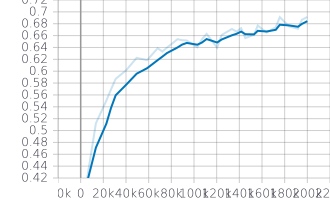
\includegraphics[width=6cm]{./Bilder/eval/mAP.png} % hier die svg graphiken verwenden
%         \subcaption{mAP}    
%     \end{subfigure}
%     \begin{subfigure}{6cm}
%         \centering
%         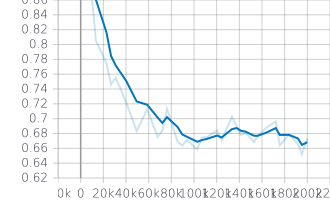
\includegraphics[width=6cm]{./Bilder/eval/loss.png}
%         \subcaption{loss}    
%     \end{subfigure}
%     \caption{Loss und mAP für 200000 Steps}
%     \label{plot:map_loss}
% \end{figure}


% % \begin{figure}[htb]
% %     \centering
% %     \begin{subfigure}{6cm}
% %         \centering
% %         \def\svgwidth{5cm}
% %         \input{./Bilder/eval/mAP.pdf_tex}
% %         %\subcaption{mAP}
% %         %\label{subfig:raspy}
% %     \end{subfigure}
% %     % \begin{subfigure}{6cm}
% %     %     \centering
% %     %     \def\svgwidth{5cm}
% %     %     \input{./Bilder/eval/loss.pdf_tex}
% %     %     %\subcaption{Loss}
% %     %     %\label{subfig:rpicam}
% %     % \end{subfigure}
% %     \label{plot:map_loss}
% % \end{figure}




% % wenn einzelnde klassen evaluiert werden können:
% % Spalten: mAP | AP classe1 | AP classe2 | ... | AP classe n



% \subsection{Graustufen/Infrarot Bilder}\label{subsec:eval_gray}

% Da, wie die Ergebnisse in \ref{subsec:regularization} und 
% \ref{subsec:distributions} gezeigt haben eine Augmentierung (welche 
% Augmentierungen) die erfogreichste Regularisierungs technik 
% war, wurde für die Graustufen Bilder nur Auf Augmentierte Bilder 
% mit faster Inception trainiert:
% \\
% hier für die drei in \ref{subsec:train_gray} verwendeten modelle 
% jwls für die in \ref{subsec:distributions} beschriebenen eval daten 
% sätze vergleichen.

% \begin{table}[htb]
%     \centering
%     \label{tab:eval_gray}
%     \begin{tabular}{| l | l || c | c |} 
%         \hline
%         Modell & Dataset & mAP & Loss\\
%         \hline
%         \multirow{2}{*}{rgb} & original & 0.6556 & 0.1451 \\
%         & handy & 0.4155 & 0.2389 \\
%         \hline
%         \multirow{2}{*}{gray 1 channel} & original & 0.5625 & 0.1716 \\
%         & handy & 0.3226 & 0.2747 \\
%         \hline
%         \multirow{2}{*}{gray 3 channel} & original & 0.664 & 0.1653 \\
%         & handy & 0.438 & 0.2492 \\
%         \hline
%     \end{tabular}        
%     \caption{Grayscale}
% \end{table}


% \begin{figure}[htb]
%     \centering
%     \begin{subfigure}{5cm}
%         \centering
%         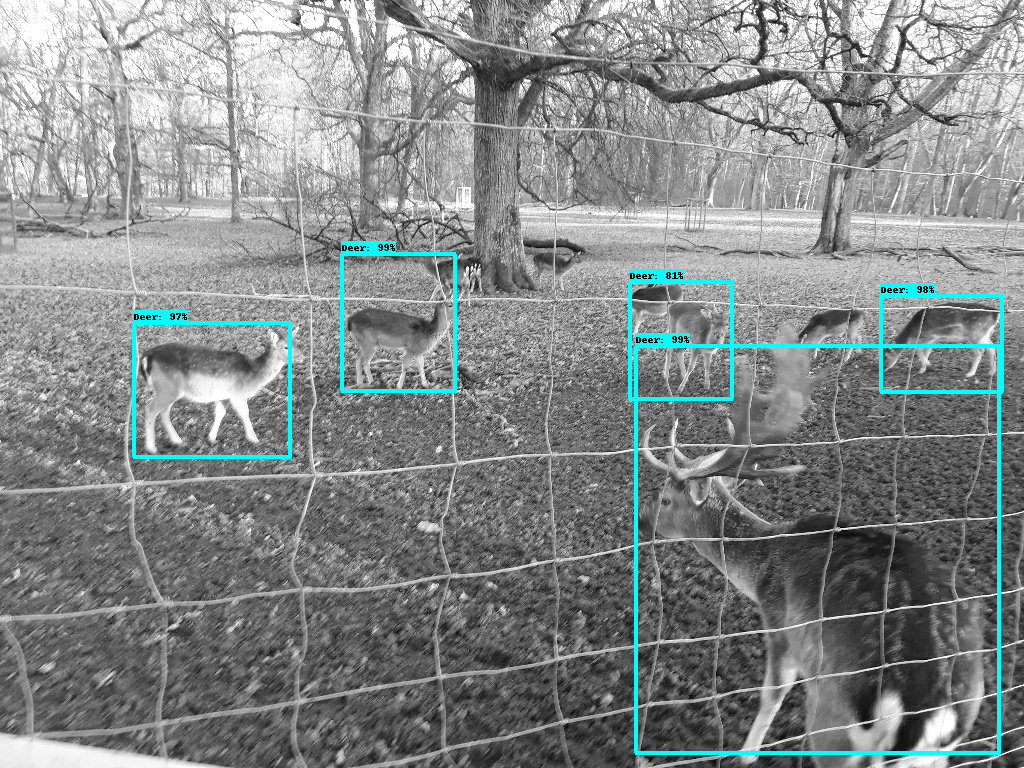
\includegraphics[width=5cm]{./Bilder/eval/rgb.png}
%         \subcaption{rbg}
%     \end{subfigure}
%     \begin{subfigure}{5cm}
%         \centering
%         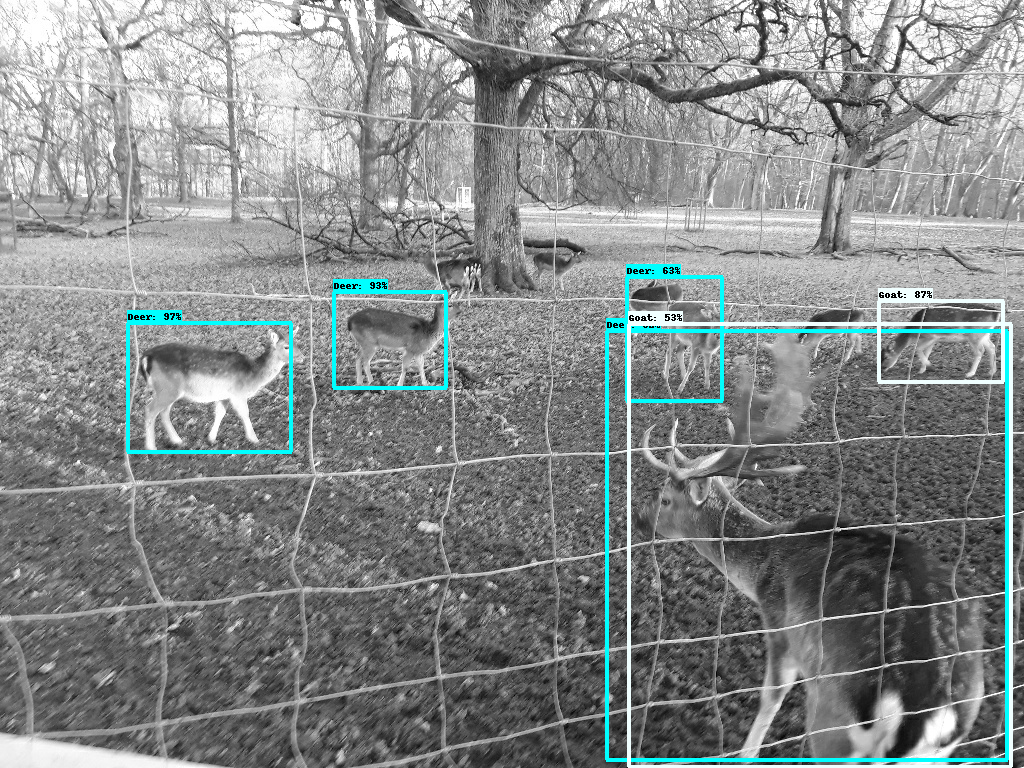
\includegraphics[width=5cm]{./Bilder/eval/gray_1ch.png}
%         \subcaption{grau (1channel)}
%     \end{subfigure}
%     \begin{subfigure}{5cm}
%         \centering
%         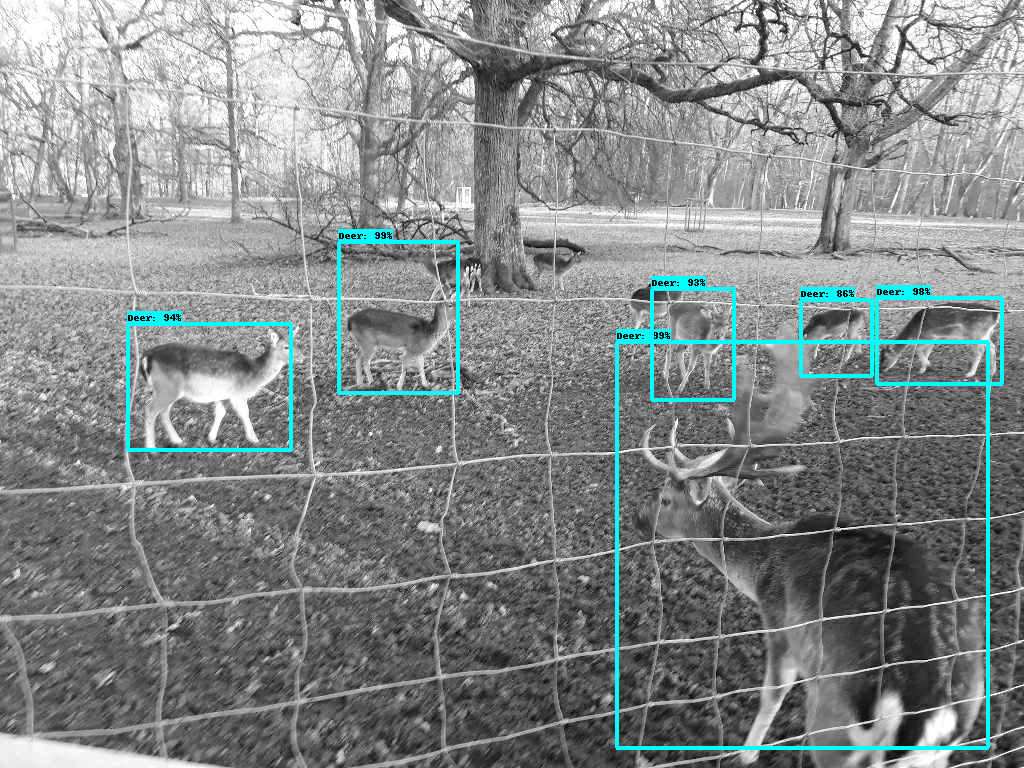
\includegraphics[width=5cm]{./Bilder/eval/gray_3ch.png}
%         \subcaption{grau (3channel)}
%     \end{subfigure}
%     \caption{Vergleich der Inferenz von grau bildern für verschiedene Modelle}
%     \label{img:raspy_cam}
% \end{figure}





% Diskussion des Ergebnisses: welchen einfluss haben Form und Farbe 
% bei training, unnötig gelernte features für gray bilder? schnelligkeit?
% \\
% Da es sich bei den convertierten graustufen bilder ja nicht um 
% echte Graustufen bilder handelt, wurden Test Bilder von Alltags gegenständen 
% mit der Für die Applikation verwendeten RaspiCam im Infrarot Modus aufgenommen. Um diese 
% \\
% (hat der Infrarot Modus mit Wärme, also lebendigkeit des Objektes zu zun??)
% \\
% Um diese Zu testen wurde ein weiteres Netz auf diese Gegenstände 
% (Gesicht, Hand, ) trainiert und im folgenden auf 
% den Datensatz true-ir evaluiert.

